% (c) 2012 Tiziana Manca - tmanca@libero.it
% (c) 2012 - 2014 Dimitrios Vrettos - d.vrettos@gmail.com

\chapter{Relazioni}
%===================================
\section{Proposizioni e predicati}
In matematica frasi come ``19 è maggiore di~5'' o ``Giove ruota intorno alla Terra'' sono considerate \emph{proposizioni} perché ad esse
si può attribuire un preciso valore di verità, cioè si può stabilire se sono vere oppure false: la prima è una proposizione vera, la seconda è falsa.

Non sono proposizioni in senso matematico ``Cosa stai studiando?'', ``domani pioverà!'', ``$x$ è un numero primo'':
infatti la prima non è un'affermazione ma pone una domanda, la seconda è una esclamazione e quindi non possiamo stabilire se è vera o falsa;
l'ultima contiene un elemento indeterminato e finché non si fissa il valore da attribuire a~$x$, non si può decidere se la frase che lo riguarda è vera o falsa.

Ogni proposizione è formata da un \emph{predicato} (verbo) e dai suoi \emph{argomenti} (cose o persone alle quali il verbo si riferisce).

Analizzando le proposizioni sopra enunciate si ha:
\begin{center}
\begin{tabular}{llc}
\toprule
Soggetto & Predicato & Complemento \\
\midrule
19 & è maggiore di & 5 \\
Giove & ruota attorno alla & Terra \\
\bottomrule
\end{tabular}
\end{center}
Il soggetto e il complemento sono gli argomenti ai quali il predicato si riferisce.
In alcune proposizioni il predicato si riferisce a due argomenti (il \emph{soggetto} e il \emph{complemento})
in altre ad un solo argomento: ad esempio, il predicato ``essere numero primo'' stabilisce semplicemente una caratteristica del numero~5
senza porre alcuna connessione con un altro argomento.

\begin{definizione}\label{def:predicato_binario}
Si dice \emph{predicato binario} un predicato che si riferisce a due argomenti.
\end{definizione}

\ovalbox{\risolvi \ref{ese:B.1}}

\section{Relazioni in un insieme}

Il termine \emph{relazione} entra molto spesso in frasi del linguaggio naturale, lo usiamo per esprimere un generico legame tra due persone o tra due oggetti,
anche senza specificarne la natura: ``si è conclusa la relazione tra Anna e Paolo'', ``l'allungamento di una sbarretta di ferro è in relazione con il calore fornito'',
``la frana del terreno è in relazione con il disboscamento della zona e l'abusivismo edilizio'', ``domani consegnerò la relazione di fisica''.
Sono tutte espressioni che ci danno informazioni di un qualche collegamento tra gli
argomenti (persone, cose) ai quali il termine relazione si riferisce.

Dal punto di vista matematico diamo la seguente definizione.
\begin{definizione}
Si dice \emph{relazione} in un insieme~$A$ un predicato binario che lega due elementi dell'insieme.
\end{definizione}

\begin{exrig}
 \begin{esempio}
 Nell'insieme~$A = \{3\text{,~}5\text{,~}6\text{,~}9\text{,~}30\}$ è introdotto il predicato binario ``essere multiplo di''; con esso formiamo le proposizioni vere scegliendo soggetto e
 complemento nell'insieme~$A$:

\begin{multicols}{3}
30 è multiplo di~6;

9 è multiplo di~3;

30 è multiplo di~3;

6 è multiplo di~3;

30 è multiplo di~5;

3 è multiplo di~3;

5 è multiplo di~5;

6 è multiplo di~6;

9 è multiplo di~9;

30 è multiplo di~30.
\end{multicols}
Il predicato ``essere multiplo'' genera nell'insieme~$A$ una relazione matematica. Esso tuttavia non è il
solo che permette di collegare tra loro due elementi di quell'insieme.
\end{esempio}
\end{exrig}

\ovalbox{\risolvi \ref{ese:B.2}}

Se chiamiamo con~$\Rel$ il predicato binario che definisce la relazione introdotta nell'insieme, per indicare 
sinteticamente la proposizione avente come soggetto~$a$, come complemento~$b$ e come predicato~$\Rel$, scriviamo~$a \,\Rel\, b$ e
diremo che~\emph{$a$ è in relazione con~$b$}.

\begin{exrig}
 \begin{esempio}

Con riferimento all'esempio precedente si ha:~$A = \{3\text{,~}5\text{,~}6\text{,~}9\text{,~}30\}$ e $\Rel$:
``essere multiplo di''. Allora scriviamo: per qualunque~$a$ e~$b$ appartenenti ad~$A$,
$a \,\Rel\, b$ se e solo se~$a$ è multiplo di~$b$, in particolare:
\[30 \,\Rel\,~6;\quad~9 \,\Rel\,~3;\quad~30 \,\Rel\,~3;\quad~6 \,\Rel\,~3;\quad~30 \,\Rel\,~5;\quad~3 \,\Rel\,~3;\quad 5 \,\Rel\,~5;\quad~6 \,\Rel\,~6;\quad~9 \,\Rel\,~9;\quad~30 \,\Rel\,~30.\]
\end{esempio}
\end{exrig}

Abbiamo così formato un insieme di coppie ordinate di elementi tra loro in relazione:~$30 \,\Rel\,~5$ può anche essere indicata con la coppia ordinata~$(30;5)$.

\begin{definizione}
Chiamiamo \emph{insieme della relazione} $G_\Rel$ l'insieme delle coppie ordinate i cui
elementi sono gli argomenti del predicato binario, ossia sono in relazione tra di loro. Esso risulta essere un
sottoinsieme del prodotto cartesiano dell'insieme~$A$ con se stesso. Si rappresenta per proprietà caratteristica nel
seguente modo~$G_\Rel = \{(a;b) \in A \times A \mid  a \,\Rel\, b \}$.
\end{definizione}

\ovalbox{\risolvii \ref{ese:B.3}, \ref{ese:B.4}, \ref{ese:B.5}, \ref{ese:B.6}}
%===================================
\subsection{Grafico di una relazione}

Dal momento che una relazione in un insieme~$Y$ determina un sottoinsieme del prodotto cartesiano~$Y \times Y$, è
comodo rappresentare una relazione nello stesso diagramma usato per rappresentare il prodotto cartesiano.
Una relazione può quindi essere rappresentata attraverso un \emph{grafico cartesiano}.

\ovalbox{\risolvii \ref{ese:B.7}, \ref{ese:B.8}}

%===================================
\subsection{Matrice o tabella di una relazione}

Nella figura~\ref{fig:B.1} è rappresentata la classica griglia per il gioco della battaglia navale.
Ogni cella è individuata da una coppia ordinata il cui primo elemento (una lettera dell'alfabeto) indica la riga,
il secondo (un numero) indica la colonna; così la coppia~$(D;5)$ indica la cella annerita.

\ovalbox{\risolvii \ref{ese:B.9}, \ref{ese:B.10}, \ref{ese:B.11}}

%===================================
\subsection{Grafo di una relazione}

\begin{definizione}
Un \emph{grafo} è un insieme di punti, detti \emph{nodi}, e di archi che uniscono coppie di punti.
\end{definizione}

Abbiamo visto che con un predicato si possono formare alcune proposizioni aventi rispettivamente come soggetto e
come complemento elementi di un insieme: solo le proposizioni vere determinano la relazione tra gli elementi di
quell'insieme e generano coppie di elementi in relazione.

\begin{exrig}
 \begin{esempio}

Nel diagramma di Eulero-Venn di figura~\ref{fig:B.2}, relativo all'insieme~$A = \{$3, 5, 6, 9, 30$\}$
rappresentiamo la relazione~$\Rel$ = ``essere multiplo di'' collegando, mediante una freccia, gli argomenti delle proposizione vere.

Come puoi osservare, l'elemento~30 è collegato con una freccia all'elemento~6 in quanto la proposizione ``30 è multiplo di~6'' è vera, ma non all'elemento~9
poiché la proposizione ``30 è multiplo di~9'' è falsa; inoltre la punta della freccia è sul numero~6 in quanto complemento del predicato ``essere multiplo di'' (si parla in tal caso di \emph{grafo orientato});
infine su ciascun elemento abbiamo messo un ``anello'' o ``cappio'' per indicare che ogni elemento è in relazione con se stesso visto che per ogni
elemento~$a \in A$ la proposizione ``$a$ è multiplo di~$a$'' risulta vera.

 \end{esempio}
\end{exrig}

\ovalbox{\risolvii \ref{ese:B.12}, \ref{ese:B.13}, \ref{ese:B.14}, \ref{ese:B.15}, \ref{ese:B.16}, \ref{ese:B.17}, \ref{ese:B.18}}
\begin{figure}[hb]
\begin{minipage}[t]{.45\textwidth}
 \centering
 % (c) 2012 Dimitrios Vrettos - d.vrettos@gmail.com

\begin{tikzpicture}[x=10mm,y=10mm, font=\small,table nodes/.style={%
		rectangle,
		draw=black,
 		align=center,
   		minimum height=5mm,
     	text depth=0.5ex,
     	text height=1.5ex,
     	inner xsep=-1pt,
     	outer sep=0pt
	},
	table/.style={%
        matrix of nodes,
        row sep=-\pgflinewidth,
        column sep=-\pgflinewidth,
        nodes={%
            table nodes
        },
        execute at empty cell={\node[fill=black]{};}
    }]

\matrix (first) [table,text width=7mm,name=table]
{
{}  & 1 & 2 & 3 &4 & 5 & 6 & 7\\
$A$ &{} &{} &{} &{} &{} &{} &{} \\
$B$ &{} &{} &{} &{} &{} &{} &{} \\
$C$ &{} &{} &{} &{} &{} &{} &{} \\
$D$ &{} &{} &{} &{} & &{} &{}  \\
$E$ &{} &{} &{} &{} &{} &{} &{} \\
$F$ &{} &{} &{} &{} &{} &{} &{} \\
};

\end{tikzpicture}

 \caption{Griglia della battaglia navale.}\label{fig:B.1}
\end{minipage}\hfil
\begin{minipage}[t]{.45\textwidth}
 \centering
 % (c) 2012 Dimitrios Vrettos - d.vrettos@gmail.com

\begin{tikzpicture}[x=10mm,y=10mm, font=\small, every state/.style={draw=CornflowerBlue}, every loop/.style={draw=Maroon}]
\draw (0,0) circle (2);

\node[state] (5) at (-1.5,0) {5};
\node[state] (30) at (-.4,.8) {30};
\node[state] (6) at (1.1,.5) {6};
\node[state] (9) at (1,-1) {9};
\node[state] (3) at (-.5,-1.2) {3};

\begin{scope}[->]
\path(5) edge[loop below] node{} ()
	(30) edge[loop above] node{} ()
	(6) edge[loop above] node{} ()
	(9) edge[loop above] node{} ()
	(3) edge[loop left] node{} ();

\end{scope}
\begin{scope}[->, Maroon]
\draw (30)--(5);
\draw (30)--(6);
\draw (30)--(3);
\draw (6)--(3);
\draw (9)--(3);
\end{scope}
\end{tikzpicture}

 \caption{L'insieme~$A$.}\label{fig:B.2}
\end{minipage}
\end{figure}

\pagebreak
\section{Proprietà delle relazioni}
%===================================
\subsection{Proprietà riflessiva}

\begin{exrig}
 \begin{esempio}

Nell'insieme~$T = \{\text{7, 8, 12, 34, 100}\}$ è introdotta la relazione~$\Rel$: ``essere divisore di''.
Puoi verificare che ogni numero è divisore di se stesso, cioè ogni elemento dell'insieme è in relazione
con se stesso. Una relazione di questo tipo si dice che gode della \emph{proprietà riflessiva}.
Osserva, però, che nell'insieme ~$\insN$ dei numeri naturali la relazione ``essere divisibile per'' non è riflessiva poiché zero non è divisibile per se stesso.
 \end{esempio}
\end{exrig}

\begin{definizione}
Una relazione~$\Rel$ in un insieme~$A$ gode della \emph{proprietà riflessiva} quando ogni elemento è in relazione con se stesso, ossia per qualunque~$x$ dell'insieme~$A$ si ha~$x \,\Rel\, x$.
\end{definizione}

\ovalbox{\risolvi \ref{ese:B.19}}

%===================================
\subsection{Proprietà antiriflessiva}

\begin{exrig}
 \begin{esempio}
Nell'insieme delle persone~$P = \{\text{Marco, Antonio, Carlo}\}$ è data la relazione~$\Rel$: ``essere più alto di''
rappresentata con la figura~\ref{fig:B.3} di pagina~\pageref{fig:B.3}.
Puoi notare che nessun elemento è in relazione con se stesso. In effetti nessuno può essere più alto di se stesso.

 \end{esempio}
\end{exrig}

\begin{definizione}
Una relazione~$\Rel$ in un insieme~$A$ gode della \emph{proprietà antiriflessiva} quando nessun elemento è in relazione con se stesso,
ossia per nessun elemento~$x$ di~$A$ si ha~$x \,\Rel\, x$.
\end{definizione}

\ovalbox{\risolvi \ref{ese:B.20}}
\subsection{Proprietà simmetrica}

\begin{exrig}
 \begin{esempio}
Nella figura~\ref{fig:B.4} a pagina~\pageref{fig:B.4} è rappresentata la relazione~$\Rel$: ``essere concorde con'' nell'insieme dei numeri~$A = \{-1\text{, }+3\text{, }-7\text{, }+5\text{, }-2\text{, }+4\text{, }+10\}$.
Per collegare elementi in relazione abbiamo usato archi anziché frecce poiché, ad esempio, le proposizioni ``$+3$ è concorde con~$+10$'' e ``$+10$ è concorde con~$+3$''
sono entrambe vere. Per questa relazione si può osservare che se un elemento dell'insieme è in relazione con un altro allora anche quest'ultimo è in relazione con il primo:
$-1 \,\Rel\, -7$, ma anche~$-7 \,\Rel\, -1$; $+3 \,\Rel\, +5$, ma anche~$+5 \,\Rel\, +3$ e così via.
 \end{esempio}
\end{exrig}

\begin{figure}[ht]
\begin{minipage}[t]{.45\textwidth}
 \centering
 % (c) 2012 Dimitrios Vrettos - d.vrettos@gmail.com

\begin{tikzpicture}[x=10mm,y=10mm, font=\small, every state/.style={draw=CornflowerBlue}, every loop/.style={draw=Maroon}]
\draw (0,0) circle (1.8);

\node at (1.8,1.5) {$P$};

\node[state] (M) at (-1,.3) {$M$};
\node[state] (C) at (.8,.8) {$C$};
\node[state] (A) at (.2,-1) {$A$};

 \begin{scope}[->, Maroon]
 \draw (M)--(C);
 \draw (M)--(A);
 \draw (C)--(A);
 \end{scope}
\end{tikzpicture}
 \caption{Proprietà antiriflessiva.}\label{fig:B.3}
\end{minipage}\hfil
\begin{minipage}[t]{.45\textwidth}
 \centering
 % (c) 2012 Dimitrios Vrettos - d.vrettos@gmail.com

\begin{tikzpicture}[x=10mm,y=10mm, font=\small, every state/.style={draw=CornflowerBlue}, every loop/.style={draw=Maroon}]
\draw (0,0) circle [x radius=3, y radius=2];

\node[state] (A) at (-2.3,.3) {$-1$};
\node[state] (B) at (-.8,1.2) {$-2$};
\node[state] (C) at (-1.5,-1) {$-7$};
\node[state] (D) at (-.5,-.9) {$+10$};
\node[state] (E) at (.6,.9) {$+3$};
\node[state] (F) at (1.8,.5) {$+4$};
\node[state] (G) at (1.5,-1) {$+5$};

\begin{scope}[->]
\path(A) edge[loop below] node{} ()
	(B) edge[loop right] node{} ()
	(C) edge[loop left] node{} ()	
(D) edge[loop below] node{} ()
	(E) edge[loop above] node{} ()
	(F) edge[loop right] node{} ()
	(G) edge[loop right] node{} ();

\end{scope}
% \begin{scope}[<->, Maroon]
 \begin{scope}[-, Maroon]
 \draw (A)--(C);
 \draw (B)--(A);
 \draw (C)--(B);
\draw (D)--(E);
\draw (D)--(F);
\draw (E)--(F);
\draw (G)--(F);
\draw (E)--(G);
\draw (D)--(G);
 \end{scope}
\end{tikzpicture}

 \caption{Proprietà simmetrica.}\label{fig:B.4}
\end{minipage}
\end{figure}

\begin{definizione}
Una relazione~$\Rel$ in un insieme~$A$ gode della \emph{proprietà simmetrica} quando risultano vere le due proposizioni
che si ottengono scambiando soggetto e complemento; ossia per qualunque~$x$ e~$y$ appartenenti all'insieme~$A$ se vale~$x \,\Rel\, y$
allora vale anche~$y \,\Rel\, x$.
\end{definizione}

\ovalbox{\risolvi \ref{ese:B.21}}

%===================================
\subsection{Proprietà antisimmetrica}

\begin{exrig}
 \begin{esempio}

Il diagramma di Venn nella figura~\ref{fig:B.5} rappresenta un insieme~$U$ e alcuni suoi sottoinsiemi.

Consideriamo ora l'insieme di insiemi~$S = \{U\text{,~}A\text{,~}B\text{,~}C\text{,~}D\text{,~}E\text{,~}F\}$ e la relazione~$\Rel$: ``essere sottoinsieme proprio di''.
Completa il grafo della relazione.

Certamente nel completare il grafo (figura~\ref{fig:B.6}) non avrai usato archi poiché è evidente che le proposizioni ``$B$ è sottoinsieme proprio di~$C$'' e ``$C$
è sottoinsieme proprio di~$B$'' non possono essere entrambe vere. Anzi, la verità della prima implica necessariamente la falsità della seconda.
 \end{esempio}
\end{exrig}

\begin{figure}[hb]
\begin{minipage}[b]{.45\textwidth}
 \centering
 % (c) 2012 Dimitrios Vrettos - d.vrettos@gmail.com

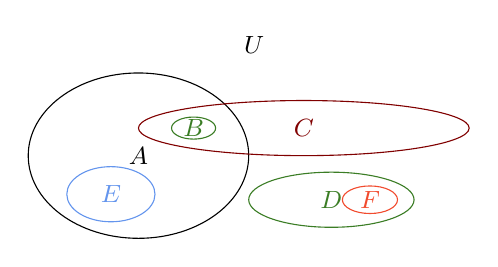
\begin{tikzpicture}[scale=.7,x=10mm,y=10mm, font=\small, every state/.style={draw=CornflowerBlue}, every loop/.style={draw=Maroon}]
\draw (0,0) circle [x radius=2, y radius=1.5] node {$A$};
\draw[CornflowerBlue] (-.5,-.7) circle [x radius=.8, y radius=.5]node {$E$};
\draw[OliveGreen] (1,.5) circle [x radius=.4, y radius=.2]node {$B$};
\draw[Maroon] (3,.5) circle [x radius=3, y radius=.5]node {$C$};
\draw[OliveGreen] (3.5,-.8) circle [x radius=1.5, y radius=.5]node {$D$};
\draw[RedOrange] (4.2,-.8) circle [x radius=.5, y radius=.25]node {$F$};

\node () at (2.1,2) {$U$};
\end{tikzpicture}
 \caption{L'insieme~$U$.}\label{fig:B.5}
\end{minipage}\hfil
\begin{minipage}[b]{.45\textwidth}
 \centering
 % (c) 2012 Dimitrios Vrettos - d.vrettos@gmail.com

\begin{tikzpicture}[scale=.7,x=10mm,y=10mm, font=\small, every state/.style={draw=CornflowerBlue}, every loop/.style={draw=Maroon}]
\draw (0,0) circle [x radius=3, y radius=2];

\node at (3,1.5) {$S$};
\node[state] (A) at (-2.3,.3) {$A$};
\node[state] (B) at (-.8,1.2) {$B$};
\node[state] (C) at (-1.5,-1) {$C$};
\node[state] (D) at (-.2,-1.1) {$D$};
\node[state] (E) at (.6,.9) {$E$};
\node[state] (F) at (1.8,.5) {$F$};
\node[state] (U) at (1.5,-1) {$U$};

  \begin{scope}[->, Maroon]
 \draw (A)--(U);
  \draw (B)--(C);
 \draw (F)--(U);
   \end{scope}
\end{tikzpicture}
 \caption{L'insieme~$S$.}\label{fig:B.6}
\end{minipage}
\end{figure}

\begin{definizione}
Una relazione~$\Rel$ in un insieme~$A$ gode della \emph{proprietà antisimmetrica} quando non possono essere vere
contemporaneamente le proposizioni che si ottengono scambiando il soggetto con il complemento, se soggetto e complemento sono diversi
tra loro; ossia per qualunque~$x$ e~$y$ dell'insieme~$A$ se~$x \neq y$ e se~$x \,\Rel\, y$ non è vero che~$y \,\Rel\, x$.
\end{definizione}

\ovalbox{\risolvi \ref{ese:B.22}}

%===================================
\subsection{Proprietà transitiva}

\begin{exrig}
 \begin{esempio}

Nel grafo di figura~\ref{fig:B.7} è rappresentata una relazione~$\Rel$ introdotta in un insieme~$T$. Dall'analisi della situazione rappresentata possiamo
affermare che dalla verità di $a \,\Rel\, b$ e~$b \,\Rel\, c$ segue la verità di~$a \,\Rel\, c$. Analizzando gli altri elementi, 
possiamo osservare che essendo vere $e \,\Rel\, f$ e~$f\, \Rel\, g$ è vera anche~$e \,\Rel\, g$;
inoltre si ha che essendo vera $n \,\Rel\, m$ e~$m \,\Rel\, t$ è vera anche~$n \,\Rel\, t$.
 \end{esempio}
\end{exrig}

\begin{figure}[ht]
\begin{minipage}[b]{.45\textwidth}
 \centering
 % (c) 2012 Dimitrios Vrettos - d.vrettos@gmail.com

\begin{tikzpicture}[x=10mm,y=10mm, font=\small, every state/.style={draw=CornflowerBlue}, every loop/.style={draw=Maroon}]
\draw (0,0) circle [x radius=3, y radius=2];

\node at (3,1.5) {$T$};
\node[state] (A) at (-2.3,.3) {$a$};
\node[state] (B) at (-.8,1.2) {$b$};
\node[state] (C) at (-1,0) {$c$};
\node[state] (G) at (.2,0) {$g$};
\node[state] (E) at (.6,1.3) {$e$};
\node[state] (F) at (1.8,.8) {$f$};
\node[state] (M) at (1.5,-1.1) {$m$};
\node[state] (N) at (0,-1.2) {$n$};
\node[state] (T) at (2.2,-.2) {$t$};
\begin{scope}[->, Maroon]
\draw (A)--(C);
\draw (B)--(C);
\draw (A)--(B);

\draw (E)--(F);
\draw (E)--(G);
\draw (F)--(G);

\draw (N)--(M);
\draw (N)--(T);
\draw (M)--(T);
\end{scope}
\end{tikzpicture}
 \caption{L'insieme~$T$.}\label{fig:B.7}
\end{minipage}\hfil
\begin{minipage}[b]{.45\textwidth}
 \centering
 % (c) 2012 Dimitrios Vrettos - d.vrettos@gmail.com

\begin{tikzpicture}[x=10mm,y=10mm, font=\small, every state/.style={draw=CornflowerBlue}, every loop/.style={draw=Maroon}]
\draw (0,0) circle [x radius=3, y radius=2];

\node at (3,1.5) {$B$};
\node[state] (A) at (-2.3,.3) {$a$};
\node[state] (H) at (-.8,1.2) {$h$};
\node[state] (F) at (-1.5,-1) {$f$};
\node[state] (B) at (-.5,-.3) {$b$};
\node[state] (E) at (.6,.9) {$e$};
\node[state] (C) at (1.8,.5) {$c$};
\node[state] (D) at (1.5,-.5) {$d$};
\node[state] (G) at (.5,-1.3) {$g$};
\begin{scope}[->]
\path(A) edge[loop below] node{} ()
(H) edge[loop right] node{} ()
(F) edge[loop left] node{} ()	
(B) edge[loop below] node{} ()
(E) edge[loop above] node{} ()
(C) edge[loop right] node{} ()
(D) edge[loop right] node{} ()
(G) edge[loop above] node{} ();
\end{scope}
\begin{scope}[-, Maroon]
\draw (A)--(H);
\draw (F)--(A);
\draw (F)--(H);
\draw (B)--(E);
\draw (B)--(C);
\draw (E)--(C);
\draw (G)--(D);
\end{scope}
\end{tikzpicture}
 \caption{L'insieme~$B$.}\label{fig:B.8}
\end{minipage}
\end{figure}

\begin{definizione}
Una relazione~$\Rel$ in un insieme~$A$ gode della \emph{proprietà transitiva} quando se~$a \,\Rel\, b$ e~$b \,\Rel\, c$
allora risulta anche~$a \,\Rel\, c$, con~$a$, $b$, $c$ elementi qualsiasi dell'insieme~$A$.
\end{definizione}

\ovalbox{\risolvii \ref{ese:B.23}, \ref{ese:B.24}, \ref{ese:B.25}, \ref{ese:B.26}, \ref{ese:B.27}, \ref{ese:B.28}, \ref{ese:B.29}}

%===================================
\section{Relazioni di equivalenza}

\begin{exrig}
 \begin{esempio}

Completa la seguente tabella segnando le proprietà di cui gode (R=riflessiva, S=simmetrica, T=transitiva) ciascuna relazione indicata.

\begin{center}
\begin{tabular}{lcc}
\toprule
Relazione & Insieme & Proprietà \\
\midrule
Avere lo stesso perimetro & poligoni & \boxR\quad\boxS\quad\boxT \\
Essere fratello di & persone & \boxR\quad\boxS\quad\boxT \\
Essere figlio di & persone & \boxR\quad\boxS\quad\boxT \\
Essere più alto di & persone & \boxR\quad\boxS\quad\boxT \\
Avere gli angoli rispettivamente congruenti & triangoli & \boxR\quad\boxS\quad\boxT \\
Iniziare con la stessa lettera & parole & \boxR\quad\boxS\quad\boxT \\
Giocare nella stessa squadra & calciatori & \boxR\quad\boxS\quad\boxT \\
$(a;b) \,\Rel\, (x;y)$ se e solo se~$a+b=x+y$ & ~$\insN \times \insN$ & \boxR\quad\boxS\quad\boxT \\
\bottomrule
\end{tabular}
\end{center}

\emph{Svolgimento}: La prima relazione gode delle tre proprietà riflessiva, simmetrica e transitiva; infatti:

\begin{itemize*}
\item ``il poligono~$P$ ha lo stesso perimetro di se stesso'' è vera per qualunque poligono (\emph{proprietà riflessiva});
\item ``il poligono~$P_1$ ha lo stesso perimetro del poligono~$P_2$'' implica la verità della proposizione ``il
poligono~$P_2$ ha lo stesso perimetro di~$P_1$'', qualunque siano i due poligoni~$P_1$ e~$P_2$ (\emph{proprietà
simmetrica});
\item se ``il poligono~$P_1$ ha lo stesso perimetro di~$P_2$'' e ``$P_2$ ha lo stesso perimetro di~$P_3$'' allora si ha anche che ``$P_1$ ha lo stesso
perimetro di~$P_3$'', qualunque siano i poligoni~$P_1$, $P_2$, $P_3$ (\emph{proprietà transitiva}).
\end{itemize*}

Verifica tu se anche le altre relazioni godono delle tre proprietà riflessiva, simmetrica, transitiva, come
``essere fratello di'', ``avere gli angoli rispettivamente uguali'', ``iniziare con la stessa lettera''.
 \end{esempio}
\end{exrig}

\begin{definizione}
Chiamiamo \emph{relazione d'equivalenza} una relazione che gode delle tre proprietà riflessiva, simmetrica e transitiva.
\end{definizione}

\ovalbox{\risolvii \ref{ese:B.30}, \ref{ese:B.31}}

\begin{exrig}
 \begin{esempio}

Dato l'insieme~$B = \{a\text{, }b\text{, }c\text{, }d\text{, }e\text{, }f\text{, }g\text{, }h\}$ e la relazione rappresentata dal grafo di figura~\ref{fig:B.8} a pagina~\pageref{fig:B.8}, costruiamo alcuni suoi sottoinsiemi seguendo le istruzioni:
\begin{itemize*}
\item \emph{ripeti \ldots{}};
\item scegliamo a caso un elemento di~$B$;
\item formiamo un sottoinsieme contenente l'elemento scelto e tutti gli altri che con quello sono in relazione;
\item \emph{\ldots{} finché} non abbiamo esaurito tutti gli elementi.
\end{itemize*}


\emph{Svolgimento}:
\begin{itemize*}
\item scegliamo l'elemento~$a$ e definiamo il sottoinsieme~$B_1$ avente come elementi~$a$, $h$, $f$ che sono in relazione con~$a$:~$B_1 = \{a\text{, }h\text{, }f\}$.
Gli elementi di~$B$ non sono esauriti, quindi ripetiamo i passi scegliendo un elemento tra quelli rimasti;
\item scegliamo~$g$ e formiamo il sottoinsieme~$B_2$ avente come elementi~$g$ e~$d$, l'unico che con esso è in relazione:~$B_2 = \{g\text{, }d\}$.
Gli elementi dell'insieme~$B$ non sono esauriti, quindi ripetiamo i passi scegliendo un elemento tra quelli rimasti;
\item scegliamo~$c$ e formiamo il sottoinsieme~$B_3$ avente come elementi~$c$, $e$, $b$ che con esso sono in relazione:~$B_3 = \{c\text{, }e\text{, }b\}$.
\end{itemize*}

Gli elementi dell'insieme assegnato sono stati esauriti. Abbiamo così ottenuto tre sottoinsiemi dell'insieme~$B$ (figura~\ref{fig:B.9} a pagina~\pageref{fig:B.9}) che hanno queste particolari caratteristiche:

\begin{itemize*}
\item nessuno di essi è vuoto;
\item a due a due sono disgiunti (non hanno tra loro alcun elemento in comune);
\item la loro unione è l'insieme~$B$.
\end{itemize*}
 \end{esempio}
\end{exrig}

\begin{figure}[ht]
\begin{minipage}[t]{.45\textwidth}
 \centering
 % (c) 2012 Dimitrios Vrettos - d.vrettos@gmail.com

\begin{tikzpicture}[scale=.8,x=10mm,y=10mm, font=\small, every state/.style={draw=CornflowerBlue}, every loop/.style={draw=Maroon}]
\draw (0,0) circle [x radius=3, y radius=2];

\node at (3,1.5) {$B$};
\begin{scope}[dotted]
\draw (0,2) -- (-1.5,-1.73);
\draw (0,2) -- (1.5,-1.73);
\end{scope}
\node[state] (A) at (-2.3,.3) {$a$};
\node[state] (H) at (-1,1.2) {$h$};
\node[state] (F) at (-1.8,-1) {$f$};
\node[state] (B) at (1,1) {$b$};
\node[state] (E) at (1.9,.2) {$e$};
\node[state] (C) at (1.8,-1) {$c$};
\node[state] (D) at (0,.1) {$d$};
\node[state] (G) at (0,-1.3) {$g$};

\node at (-2.5,-2) {$B_1$};
\node at (0,-2.5) {$B_2$};
\node at (2.5,-2) {$B_3$};

\end{tikzpicture}
 \caption{I sottoinsiemi dell'insieme~$B$.}\label{fig:B.9}
\end{minipage}\hfil
\begin{minipage}[t]{.45\textwidth}
 \centering
 % (c) 2012 Dimitrios Vrettos - d.vrettos@gmail.com

\begin{tikzpicture}[scale=.8,x=10mm,y=10mm, font=\small, every state/.style={draw=CornflowerBlue}, every loop/.style={draw=Maroon}]
\draw (0,0) circle [x radius=3, y radius=2];

\node at (3,1.5) {$P(B)$};
\begin{scope}[dotted]
\draw (0,2) -- (-1.5,-1.73);
\draw (0,2) -- (1.5,-1.73);
\end{scope}
\node[state] (A) at (-2.3,.3) {$a$};
\node[state] (H) at (-1,1.2) {$h$};
\node[state] (F) at (-1.8,-1) {$f$};
\node[state] (B) at (1,1) {$b$};
\node[state] (E) at (1.9,.2) {$e$};
\node[state] (C) at (1.8,-1) {$c$};
\node[state] (D) at (0,.1) {$d$};
\node[state] (G) at (0,-1.3) {$g$};

\node at (-2.5,-2) {$[a]$};
\node at (0,-2.5) {$[d]$};
\node at (2.5,-2) {$[b]$};

\end{tikzpicture}
 \caption{La partizione dell'insieme~$B$ in classi d'equivalenza.}\label{fig:B.10}
\end{minipage}
\end{figure}
\pagebreak
Premettiamo le definizioni:

\begin{definizione}
Dato un insieme $A$, suddividiamolo in un numero di sottoinsiemi~$A_1$, $A_2$, \ldots, $A_n$, detti \emph{classi}, tali che
\begin{enumeratea}
\item nessun sottoinsieme è vuoto;
\item a due a due sono disgiunti (non hanno tra loro alcun elemento in comune);
\item la loro unione è l'insieme~$A$.
\end{enumeratea}
L'insieme $P(A) = \{A_1$, $A_2$, \ldots, $A_n\}$ è detto \emph{partizione} di~$A$.
\end{definizione}

\begin{definizione}
In un insieme~$A$ dove sia stata definita una relazione d'equivalenza $\Rel$, si chiama \emph{classe d'equivalenza} ogni sottoinsieme di~$A$ contenente tutti e soli gli elementi
tra loro in relazione secondo $\Rel$.
\end{definizione}

Si viene così a determinare una partizione dell'insieme~$A$ in classi d'equivalenza, ognuna delle quali è indicata racchiudendo tra parentesi quadrate
uno degli elementi della classe considerata.
Nell'esempio sopra riportato le classi d'equivalenza sono i sottoinsiemi di~$B$ indicati con~$[a]$, $[b]$, $[d]$; la
partizione dell'insieme~$B$ in classi d'equivalenza è rappresentata con il diagramma di Eulero-Venn nella figura~\ref{fig:B.10}.

\begin{definizione}
Si chiama \emph{insieme quoziente} di un insieme~$A$ rispetto alla relazione di equivalenza~$\Rel$ in esso definita,
l'insieme i cui elementi sono le classi d'equivalenza determinate dalla relazione~$\Rel$, ovvero la partizione di~$A$ definita da~$\Rel$. L'insieme quoziente si indica con il simbolo~$A/\Rel$.
\end{definizione}

Nel caso dell'esempio precedente l'insieme quoziente~$B/\Rel$ è quello riportato nel seguente diagramma di Eulero-Venn:
\begin{center}
 % (c) 2012 Dimitrios Vrettos - d.vrettos@gmail.com

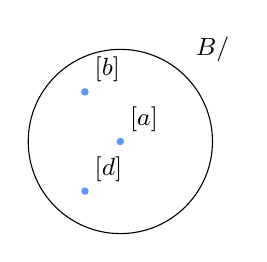
\begin{tikzpicture}[scale=.9,x=10mm,y=10mm, font=\small]
\draw (0,0) circle [x radius=1.3, y radius=1.3];

\node at (1.3,1.3) {$B/\Rel$};

\begin{scope}[fill=CornflowerBlue]
\fill  (0,0)circle (1.5pt) node[above right] {$[a]$};
\fill (-.5,.7) circle (1.5pt)node[above right] {$[b]$};
\fill(-.5,-.7) circle (1.5pt)node[above right] {$[d]$};
\end{scope}
\end{tikzpicture}

\end{center}

\osservazione Ogni volta che si ha una relazione d'equivalenza~$\Rel$ in un insieme~$A$, possiamo stabilire la seguente
catena di passaggi:
 \[\text{insieme }A\rightarrow\Rel\rightarrow\text{ partizione }P(A)=\text{ insieme quoziente }A/\Rel.\]

\ovalbox{\risolvii \ref{ese:B.32}, \ref{ese:B.33}, \ref{ese:B.34}, \ref{ese:B.35}, \ref{ese:B.36}, \ref{ese:B.37}, \ref{ese:B.38}, \ref{ese:B.39}, \ref{ese:B.40},
\ref{ese:B.41}, \ref{ese:B.42}}

\ovalbox{\ref{ese:B.43}}

\section{Relazioni di ordine}

Nel linguaggio di ogni giorno avrai certamente spesso usato espressioni come ``devo mettere in ordine i miei
libri'' oppure ``qui non c'è ordine'' e altre espressioni simili.
Anche in matematica, fin dalla scuola elementare, hai imparato a ordinare gli elementi dell'insieme dei
numeri naturali: dati due numeri naturali hai imparato infatti a stabilire quale dei due è il maggiore.

\begin{definizione}
Una relazione~$\Rel$, introdotta in un insieme~$A$, si chiama \emph{relazione d'ordine} se è antisimmetrica e transitiva.
\end{definizione}

Riguardando le varie relazioni introdotte sin qui, possiamo stabilire che esistono relazioni d'ordine di vario tipo, schematizzate nel seguente diagramma:
\begin{center}
 % (c) 2012 Dimitrios Vrettos - d.vrettos@gmail.com

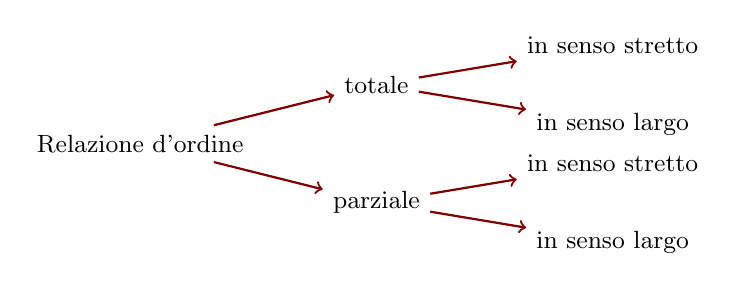
\begin{tikzpicture}[x=10mm,y=10mm, font=\small]

\node {Relazione d'ordine}[grow=right,level distance= 30mm, sibling distance=15mm,->,thick, draw=Maroon]
child {node {parziale}[sibling distance=10mm]
child {node {in senso largo}}
child {node {in senso stretto}}}
child {node {totale}[sibling distance=10mm]
child {node {in senso largo}}
child {node {in senso stretto}}};

\end{tikzpicture}

\end{center}

Attraverso alcuni esempi, vogliamo chiarire le differenze tra i diversi tipi. A questo scopo introduciamo la seguente definizione.

\begin{definizione}
Data una relazione d'ordine~$\Rel$ definita in un insieme~$A$, due elementi distinti~$x$ e~$y$ sono \emph{confrontabili} se rispetto a~$\Rel$ si ha~$x \,\Rel\, y$ oppure~$y \,\Rel\, x$.
\end{definizione}

\begin{exrig}
 \begin{esempio}

In base al diagramma di Eulero-Venn riportato nella figura~\ref{fig:B.5} a pagina~\pageref{fig:B.5}, introduciamo nell'insieme~$S = \{U$, $A$, $B$, $C$, $D$, $E$, $F\}$ la relazione~$\Rel$: ``essere sottoinsieme di''.
Ricordiamo che, dati due insiemi~$X$ e~$Y$, $X$ è \emph{sottoinsieme} di~$Y$, in simboli $X \subseteq Y$, quando ogni elemento di~$X$ appartiene a~$Y$.

Vogliamo studiare le proprietà della relazione~$\Rel$:

\begin{enumeratea}
\item poiché ogni insieme è sottoinsieme di se stesso, possiamo dire che~$\Rel$ è riflessiva;
\item se~$X \subseteq Y$ e~$X \neq Y$ allora~$Y \not\subseteq X$ quindi~$\Rel$ è una relazione antisimmetrica;
\item se~$X \subseteq Y$ e~$Y \subseteq Z$ allora~$X \subseteq Z$ quindi~$\Rel$ è una relazione transitiva.
\end{enumeratea}

Inoltre è evidente che esistono almeno due elementi dell'insieme~$S$ che non sono in
alcun modo in relazione: ad esempio~$A \not\subseteq D$ e~$D \not\subseteq A$, ossia~$A$ e~$D$ non sono confrontabili.

 \end{esempio}

 \begin{esempio}

Riprendiamo il diagramma di Eulero-Venn dell'esempio precedente e introduciamo nell'insieme~$S = \{U$, $A$, $B$, $C$, $D$, $E$, $F\}$ la relazione~$\Rel$:
``essere sottoinsieme proprio di''. Studiamo le proprietà di questa relazione:
\begin{itemize*}
 \item cosa è cambiato rispetto alla relazione precedente? $\ldots$
 \item sono ancora valide le proprietà antisimmetrica e transitiva? $\ldots$
 \item esistono elementi di~$S$ non confrontabili? $\ldots$
\end{itemize*}

 \end{esempio}
\end{exrig}

\begin{definizione}
Una relazione d'ordine si dice \emph{parziale} quando esistono almeno due elementi che non sono confrontabili.
\end{definizione}

\begin{definizione}
Una relazione d'ordine si dice \emph{totale} quando due qualsiasi elementi possono essere messi in relazione, cioè sono confrontabili.
\end{definizione}

\begin{definizione}
Una relazione d'ordine è detta \emph{in senso largo} quando essa gode della proprietà riflessiva.
\end{definizione}

\begin{definizione}
Una relazione d'ordine è detta \emph{in senso stretto} quando essa gode della proprietà antiriflessiva.
\end{definizione}

\begin{center}
 % (c) 2012 Dimitrios Vrettos - d.vrettos@gmail.com

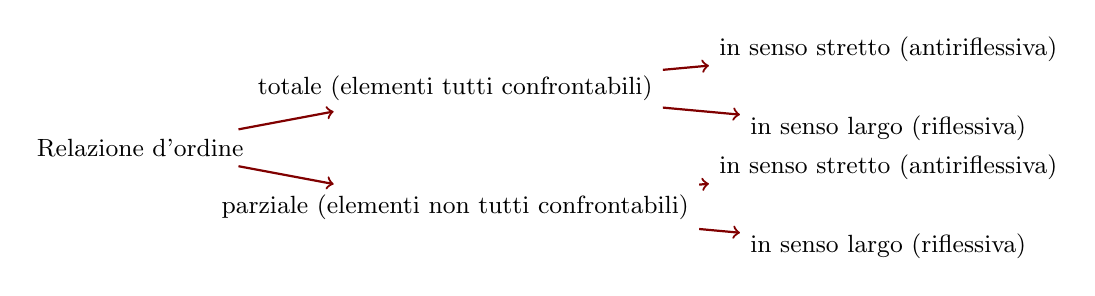
\begin{tikzpicture}[x=10mm,y=10mm, font=\small]

\node {Relazione d'ordine}[grow=right,level distance= 40mm,->,thick, draw=Maroon]
child {node {parziale (elementi non tutti confrontabili)}[level distance=55mm,sibling distance=10mm]
child {node {in senso largo (riflessiva)}}
child {node {in senso stretto (antiriflessiva)}}}
child {node {totale (elementi tutti confrontabili)}[level distance=55mm,sibling distance=10mm]
child {node {in senso largo (riflessiva)}}
child {node {in senso stretto (antiriflessiva)}}};

\end{tikzpicture}

\end{center}

\ovalbox{\risolvii \ref{ese:B.44}, \ref{ese:B.45}, \ref{ese:B.46}, \ref{ese:B.47}, \ref{ese:B.48}, \ref{ese:B.49}, \ref{ese:B.50}, \ref{ese:B.51},
\ref{ese:B.52}, \ref{ese:B.53}, \ref{ese:B.54}}

\ovalbox{ \ref{ese:B.55}, \ref{ese:B.56}, \ref{ese:B.57}, \ref{ese:B.58}, \ref{ese:B.59}, \ref{ese:B.60},
\ref{ese:B.61},\ref{ese:B.62}, \ref{ese:B.63}}
\newpage
% (c) 2012 Silvia Cibola - silvia.cibola@gmail.com
% (c) 2012 - 2014 Dimitrios Vrettos - d.vrettos@gmail.com

\section{Esercizi}

\subsection{Esercizi dei singoli capitoli}

\subsubsection*{B.1 - Prime definizioni}
\begin{esercizio}
\label{ese:B.1}
Segnate nel piano dotato di riferimento cartesiano ortogonale i vettori~$\vec{v}(1;2)$ e~$\vec{w}(3;-1)$. Possiamo affermare che~$|\vec{w}|=2 \cdot |\vec{v}|$?
\end{esercizio}

\subsubsection*{B.2 - Operazioni con i vettori}
\begin{esercizio}
\label{ese:B.2}
Provate a giustificare la seguente affermazione: l'operazione di addizione definita secondo la regola del parallelogramma gode della proprietà commutativa.
\end{esercizio}

\begin{esercizio}
\label{ese:B.3}
Determinate il vettore~$\vec{z}=\vec{u}+\vec{w}$ essendo~$\vec{u}(-1;-3)$ e~$\vec{v}(2;-1)$. Determinate inoltre il modulo di~$\vec{z}$ e la sua direzione.
Potete affermare che~$|\vec{z}|=|\vec{u}|+|\vec{w}|$?
\end{esercizio}

\begin{esercizio}
\label{ese:B.4}
Nel riferimento cartesiano ortogonale riportato di seguito sono rappresentati i vettori~$\vec{u}$ e~$\vec{v}$. Completate:

\begin{enumeratea}
\item il vettore~$\vec{u}$ è applicato all'origine e ha componenti~$\ldots$;
\item il vettore~$\vec{v}$ ha il primo estremo in~$B(\ldots;\ldots)$ e il secondo in~$\ldots$, pertanto le sue componenti sono~$\ldots$;
\item $m_{\vec{u}}=\ldots$ e~$m_{\vec{v}}=\ldots$, pertanto essi sono~$\ldots$;
\item $|\vec{u}|=\ldots$ e~$|\vec{v}|=\ldots$;
\item determinare~$r$ in modo che~$\vec{v}=r \cdot \vec{u}$.
\end{enumeratea}
\begin{center}
 % (c) 2012 Dimitrios Vrettos - d.vrettos@gmail.com

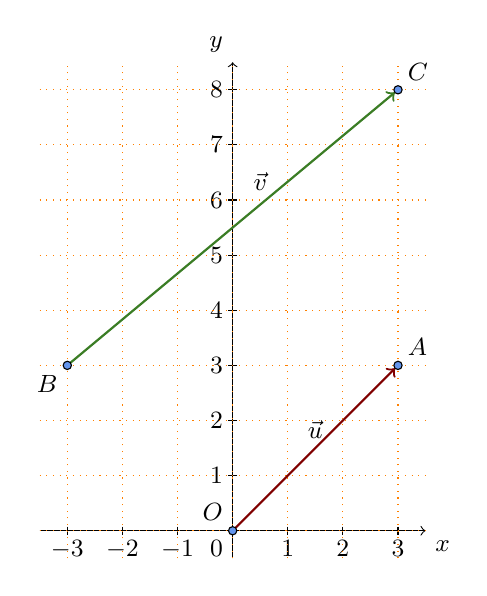
\begin{tikzpicture}[x=7mm,y=7mm, font=\small]

  \begin{scope}[->]
    \draw (-3.5,0) -- (3.5,0) node [below right] {$x$};
    \draw (0,-.5) -- (0,8.5) node[above left] {$y$};
  \end{scope}

  \foreach \x/\xtext in {-3/-3,-2/-2,-1/-1,1/1,2/2,3/3}{
    \node[below] at (\x,0) {$\xtext$};
    \draw (\x,1.5pt) -- (\x,-1.5pt);}
  \foreach \y/\ytext in {1/1,2/2,3/3,4/4,5/5,6/6,7/7,8/8}{
    \node[left] at (0,\y) {$\ytext$};
    \draw (1.5pt,\y) -- (-1.5pt,\y);}
  \node[below left] at (0,0) {$0$};

  \begin{scope}[dotted, orange, step=7mm]
    \draw (-3.5,-.5) grid (3.5,8.5);
  \end{scope}

  \begin{scope}[thick, ->,shorten >=1.5pt]
	\draw[Maroon] (0,0) -- (3,3);  
	\draw[OliveGreen](-3,3) -- (3,8);
      \end{scope}
 

\begin{scope}[fill=CornflowerBlue, draw=black]
\filldraw (0,0) circle (1.5pt)node [above left]{$O$};
\filldraw (3,3) circle (1.5pt)node [above right]{$A$};
\filldraw (-3,3) circle (1.5pt)node [below left]{$B$};
\filldraw (3,8) circle (1.5pt) node [above right]{$C$};
\end{scope}
\node[above] at (1.5,1.5) {$\vec{u}$};
\node[above] at (.5,6) {$\vec{v}$};
\end{tikzpicture}
\end{center}

\end{esercizio}

\begin{esercizio}
\label{ese:B.5}
Determinate le componenti del vettore~$\vec{w}=2 \cdot \vec{v}$ essendo~$\vec{v}(\frac{3}{2};-2)$. Verificate che~$\vec{w}$ e~$\vec{v}$ hanno stessa direzione
e~$|\vec{w}|=2 \cdot |\vec{v}|$.
\end{esercizio}

\begin{esercizio}
\label{ese:B.6}
Verificate che~$\frac{3}{2} \cdot (\vec{x}+\vec{y})=\frac{3}{2}\vec{x}+\frac{3}{2}\vec{y}$ essendo~$\vec{x}(-\frac{5}{4};1)$ e~$\vec{y}(4;-1)$.
\end{esercizio}
\pagebreak
\subsubsection*{B.3 - Dipendenza e indipendenza lineare}
\begin{esercizio}
\label{ese:B.7}
Completate le scritture:
\begin{multicols}{2}
\begin{enumeratea}
\item $\vec{v}(-\sqrt{2};\frac {5}{4})=\ldots \cdot \vec{i}+\ldots \cdot \vec{j}$;
\item $\vec{u}(1;-1)=\ldots \cdot \vec{i}+\ldots \cdot \vec{j}$;
\item $\vec{h}(\ldots;\ldots)=\frac {\sqrt{3}}{3} \cdot \vec{i}-9 \cdot \vec{j}$;
\item $\vec{z}(\ldots;\ldots)=\frac {3 \sqrt{5}}{3} \cdot \vec{i}$;
\end{enumeratea}
\end{multicols}
\end{esercizio}

\begin{esercizio}
\label{ese:B.8}
\begin{multicols}{2}
 Dati i vettori della figura a fianco, applicate il metodo geometrico per determinare i vettori che permettono di scrivere~$\vec{w}$ come combinazione lineare degli altri due.
Riprendete questi stessi vettori e determinate i vettori che permettono di scrivere~$\vec{v}$ come combinazione lineare degli altri due. In maniera analoga, determinate i vettori che permettono di scrivere~$\vec{u}$ come combinazione lineare degli altri due ($\vec{v}$ e $\vec{w}$).
\begin{center}
% (c) 2012 Dimitrios Vrettos - d.vrettos@gmail.com

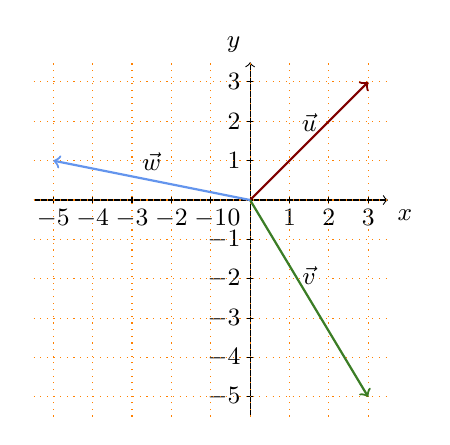
\begin{tikzpicture}[x=5mm,y=5mm, font=\small]

  \begin{scope}[->]
    \draw (-5.5,0) -- (3.5,0) node [below right] {$x$};
    \draw (0,-5.5) -- (0,3.5) node[above left] {$y$};
  \end{scope}

  \foreach \x/\xtext in {-5/-5,-4/-4,-3/-3,-2/-2,-1/-1,1/1,2/2,3/3}{
    \node[below] at (\x,0) {$\xtext$};
    \draw (\x,1.5pt) -- (\x,-1.5pt);}
  \foreach \y/\ytext in {-5/-5,-4/-4,-3/-3,-2/-2,-1/-1,1/1,2/2,3/3}{
    \node[left] at (0,\y) {$\ytext$};
    \draw (1.5pt,\y) -- (-1.5pt,\y);}
  \node[below left] at (0,0) {$0$};

  \begin{scope}[dotted, orange, step=5mm]
    \draw (-5.5,-5.5) grid (3.5,3.5);
  \end{scope}

  \begin{scope}[thick, ->]
	\draw[Maroon] (0,0) -- (3,3);  
	\draw[OliveGreen](0,0) -- (3,-5);
	\draw[CornflowerBlue] (0,0) -- (-5,1);
      \end{scope}
 
\node[above] at (1.5,1.5) {$\vec{u}$};
\node[above] at (1.5,-2.4) {$\vec{v}$};
\node[above] at (-2.5,.5) {$\vec{w}$};
\end{tikzpicture}
\end{center}
\end{multicols}
\end{esercizio}

\begin{esercizio}
\label{ese:B.9}
I vettori dell'esercizio precedente sono linearmente dipendenti?
\end{esercizio}

\begin{esercizio}
\label{ese:B.10}
Spiegate perché i tre vettori~$\vec{v}(1;2)$, $\vec{u}(3;1)$ e~$\vec{w}(-3;-6)$ sono linearmente dipendenti.
\end{esercizio}


\cleardoublepage
